\documentclass{homeworg}
\usepackage{amsmath}
\usepackage{xcolor}
\usepackage{multirow}
\title{Travail 10 - Compteur par n}
\author{Wats Raphaël}

\begin{document}
\maketitle

\section{Schématiques}

\subsection{Circuit principal}
\begin{center}
    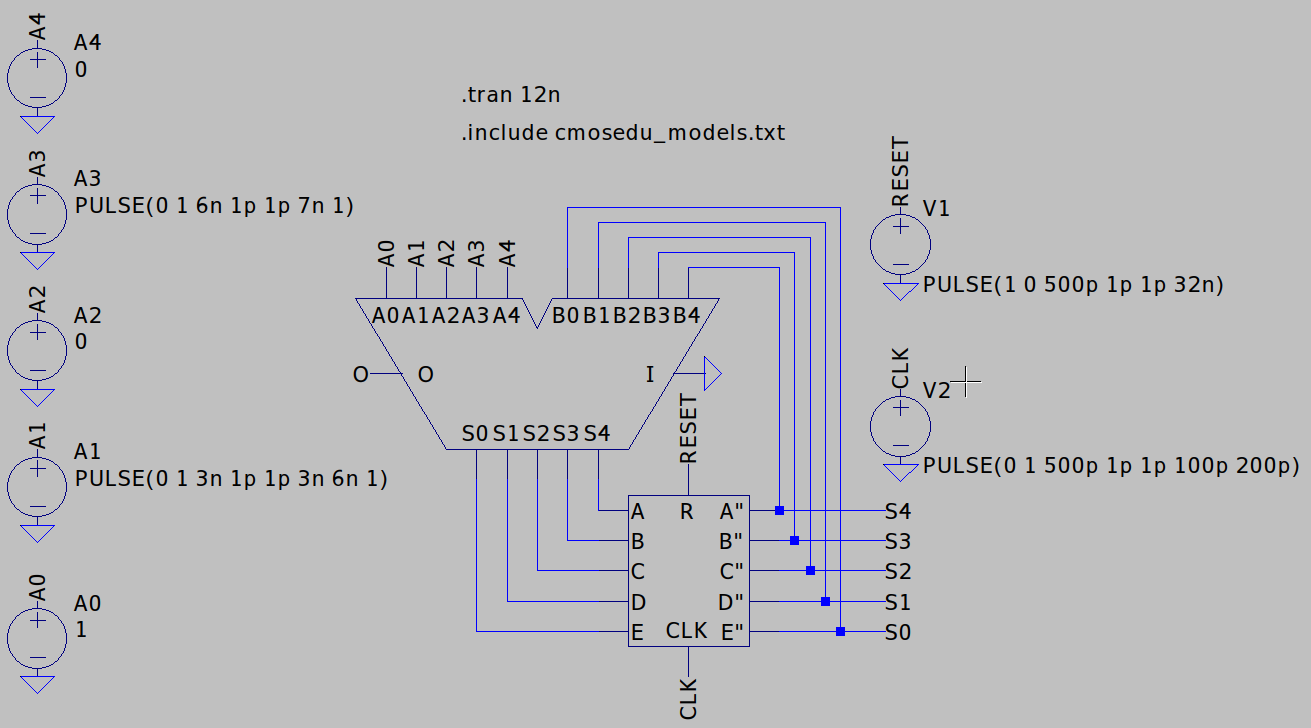
\includegraphics[scale=0.45]{main.png}
\end{center}

\newpage
\subsection{Full adder 5}
\begin{center}
    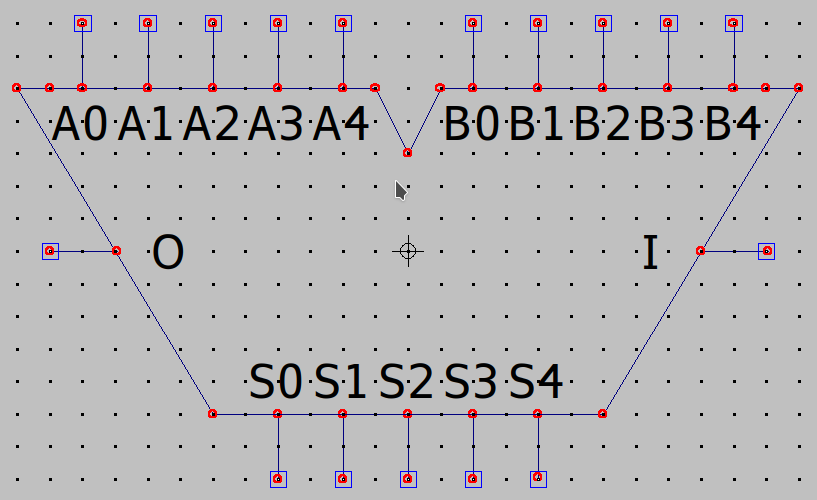
\includegraphics[scale=0.7]{fulladder5_asy.png}
    
    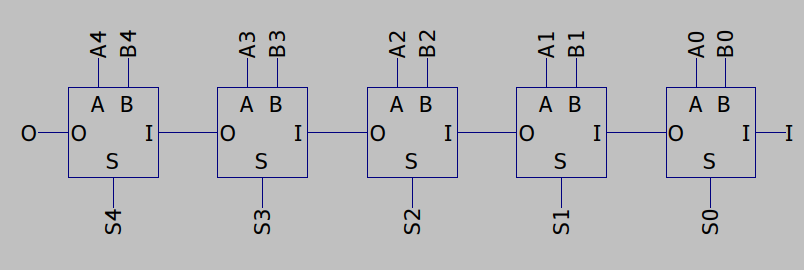
\includegraphics[scale=0.7]{fulladder5_asc.png}
\end{center}

\newpage
\subsubsection{Full adder}
    \begin{center}
        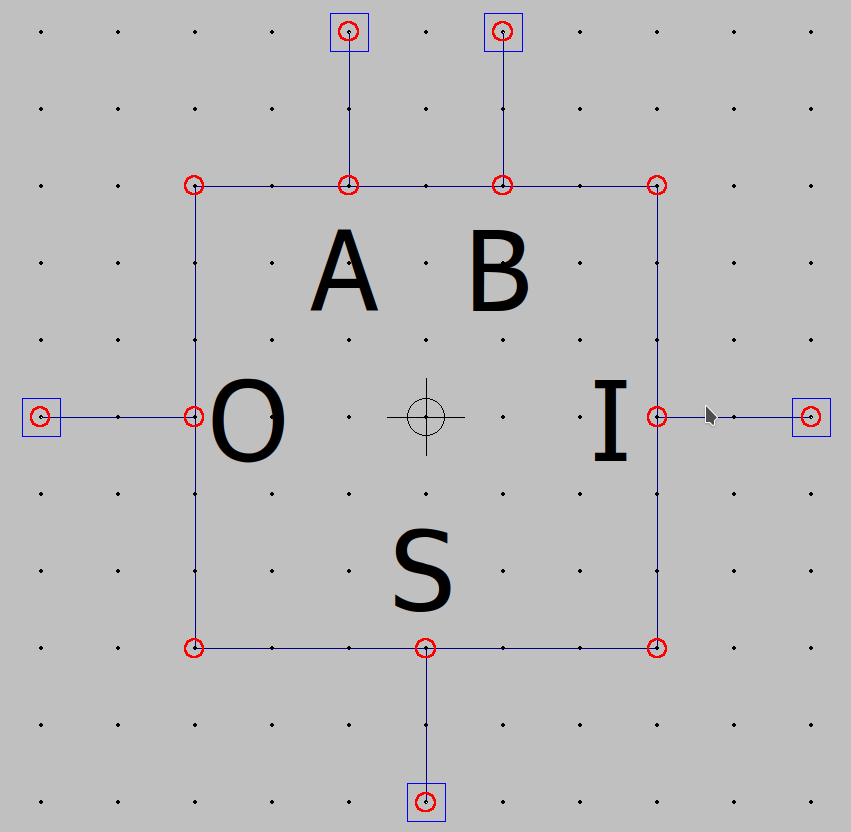
\includegraphics[scale=0.5]{fulladder_asy.png}
        
        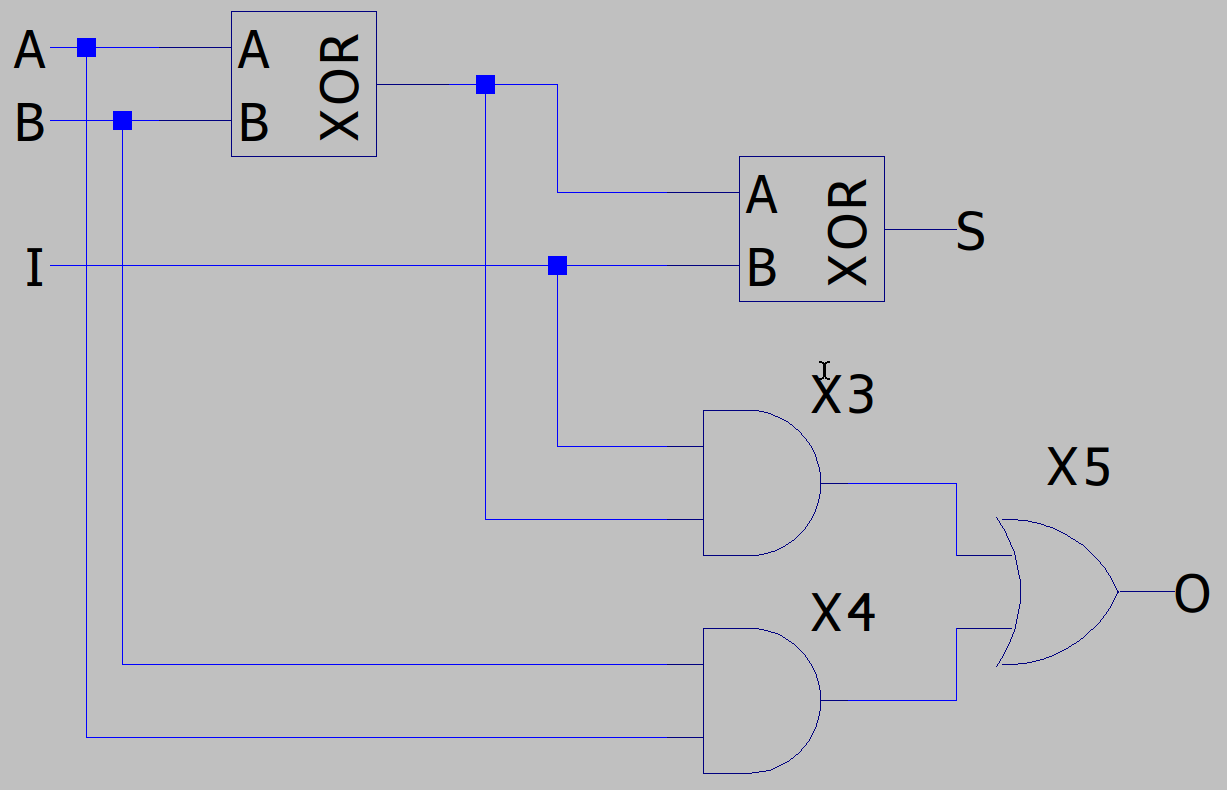
\includegraphics[scale=0.4]{fulladder_asc.png}
    \end{center}

\newpage
\paragraph{xor gate}
\begin{center}
    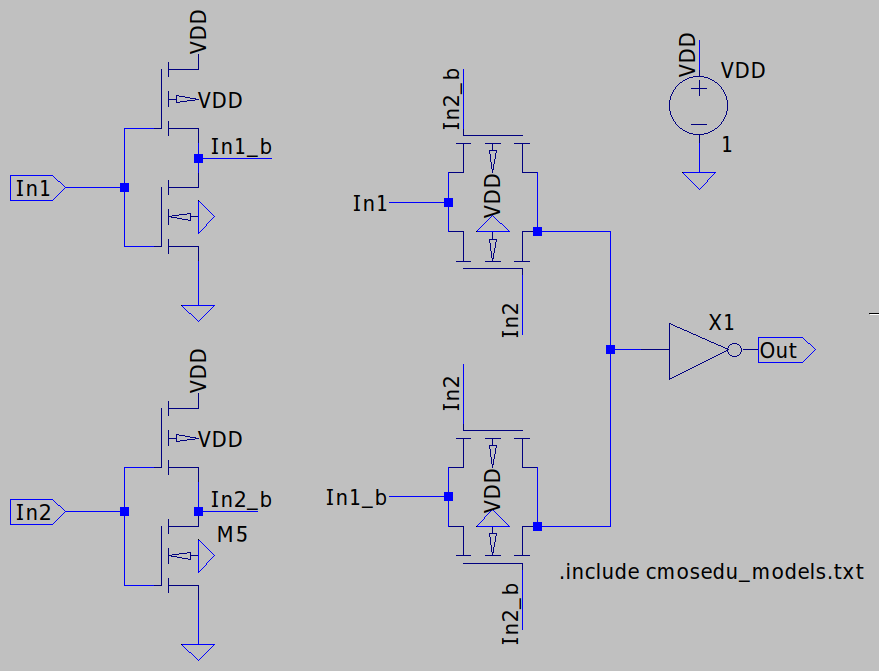
\includegraphics[scale=0.5]{xor.png}
\end{center}

\paragraph{Truth table}
\begin{center}
    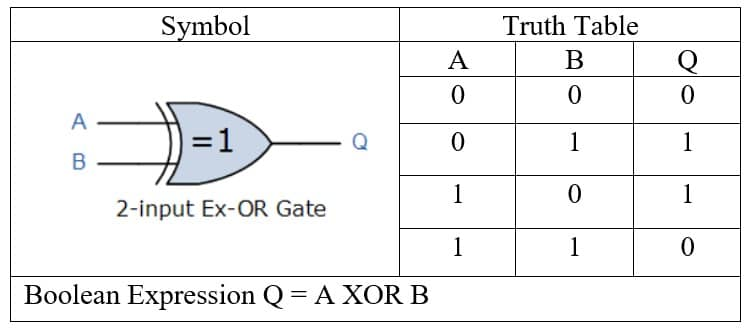
\includegraphics[scale=0.5]{XOR-Gate-truth-table.jpg}
    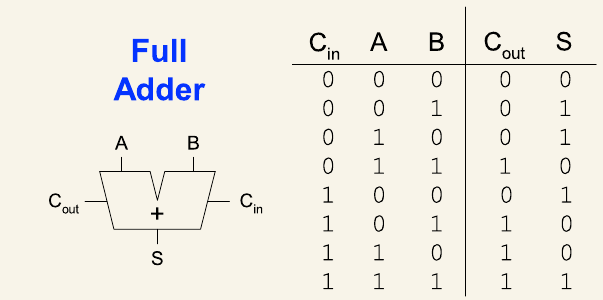
\includegraphics[scale=0.8]{fulladder_truth.png}
\end{center}

\newpage
\subsection{ddf 5 with reset}
    \begin{center}
        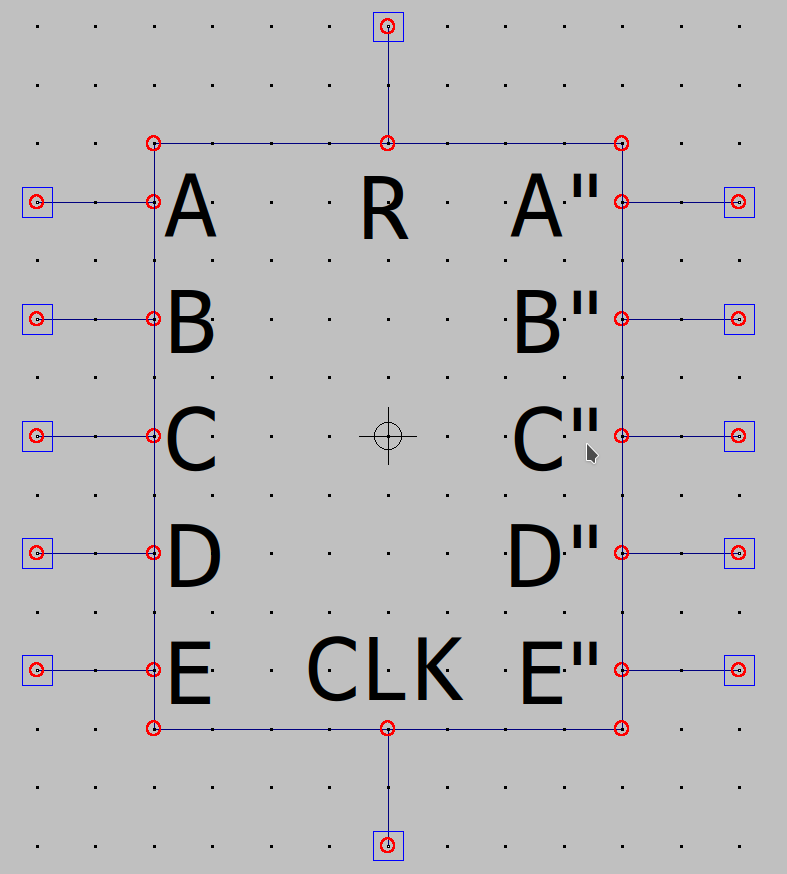
\includegraphics[scale=0.5]{dff5_reset_asy.png}
        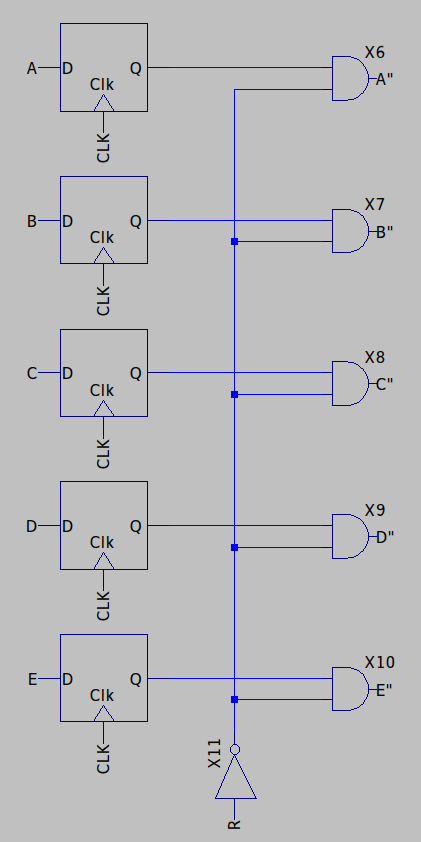
\includegraphics[scale=0.5]{dff5_reset_asc.png}
    \end{center}

\newpage
\section{Résultats de la simulation de la séquence}
    Lorsque la clock est réglé à une fréquence maximal de $500 MHz$, PULSE(0 1 2n 1p 1p 1n 2n)
    \begin{center}
        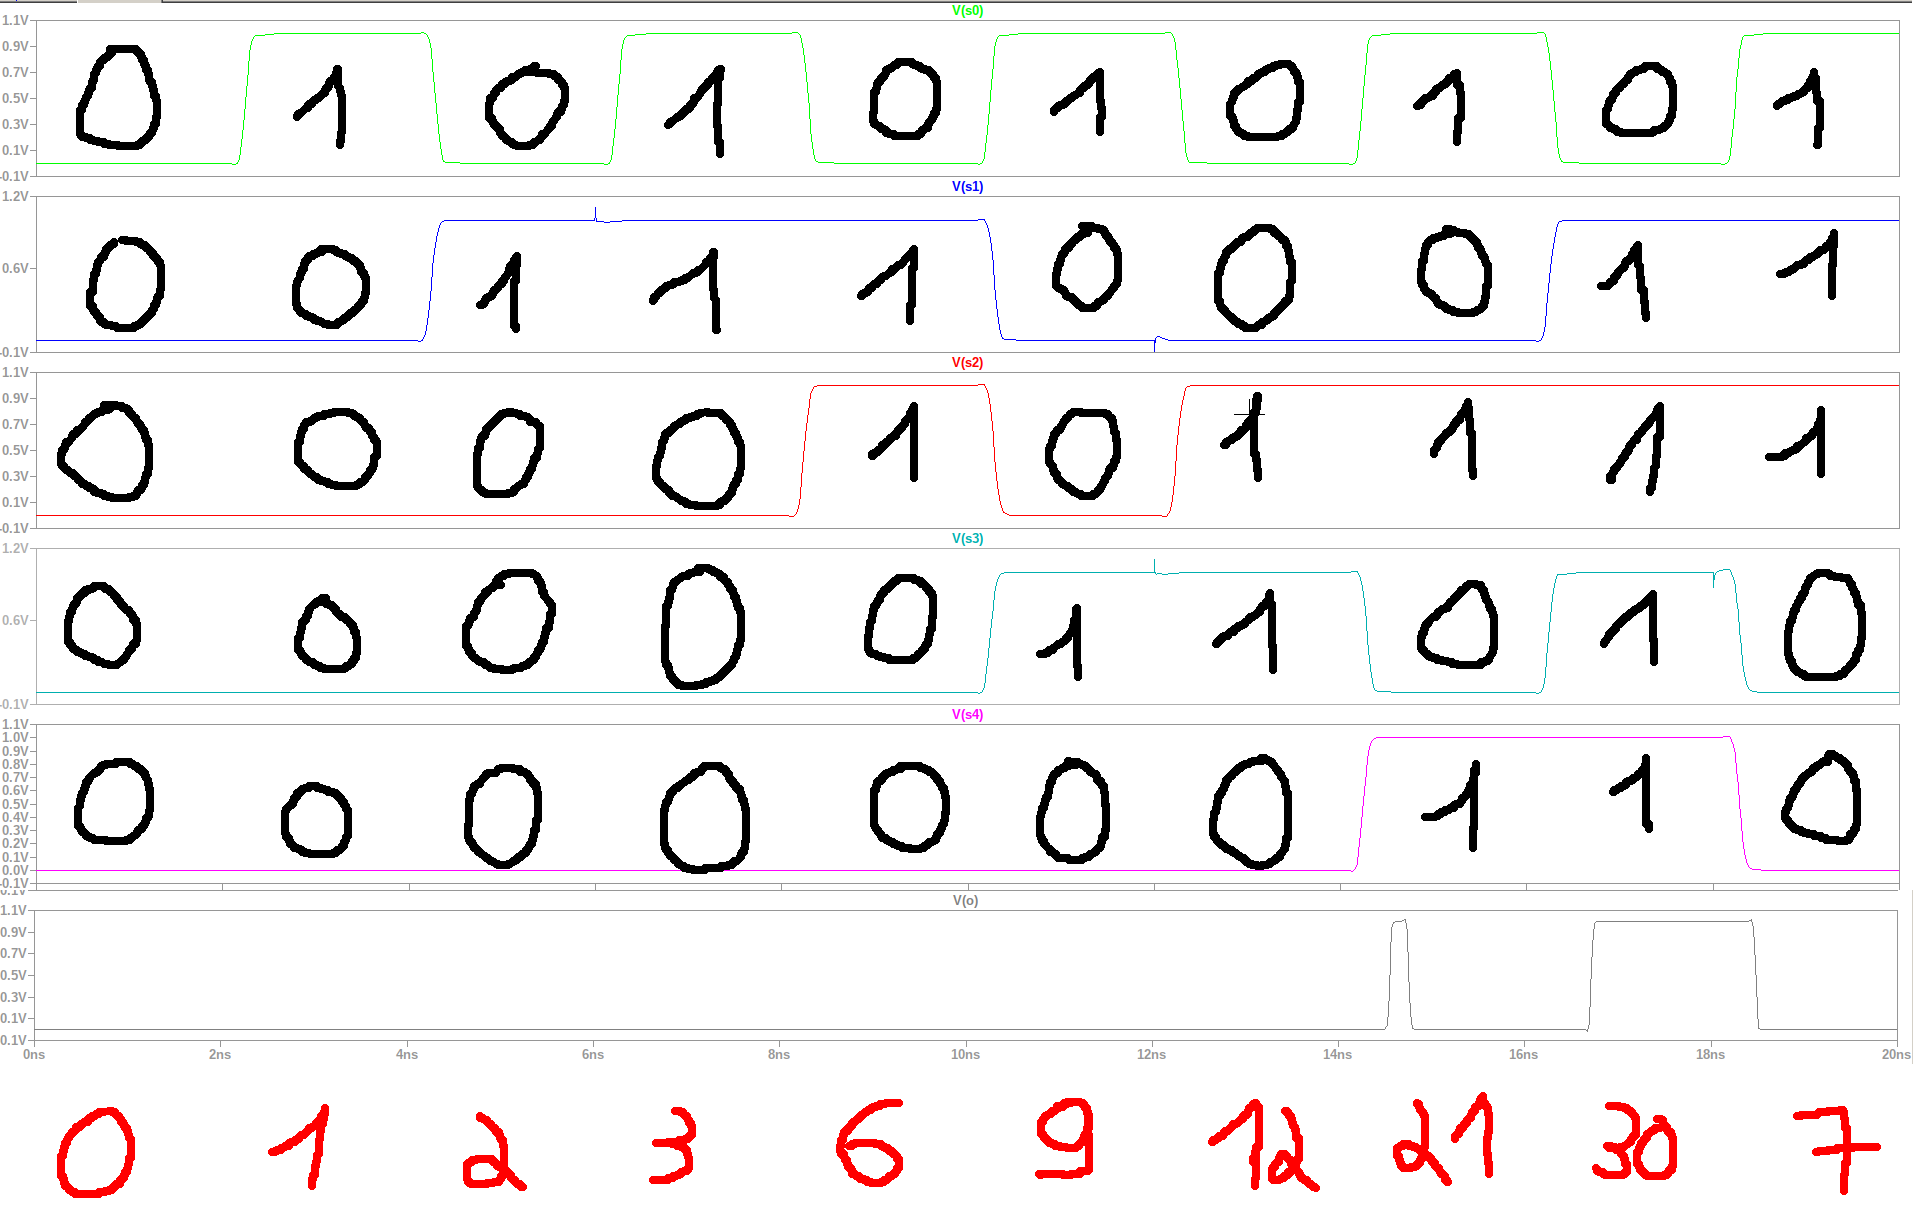
\includegraphics[scale=0.25]{count.png}
    \end{center}
    La séquence s'affiche parfaitement, Avec L'ouput à 1 lorsque l'on atteint 7 (Il y a un décalage engendré par la DFF5).
    
    Lorsque l'on double la fréquence à $1 GHz$, PULSE(0 1 1n 1p 1p 500p 1n)
    \begin{center}
        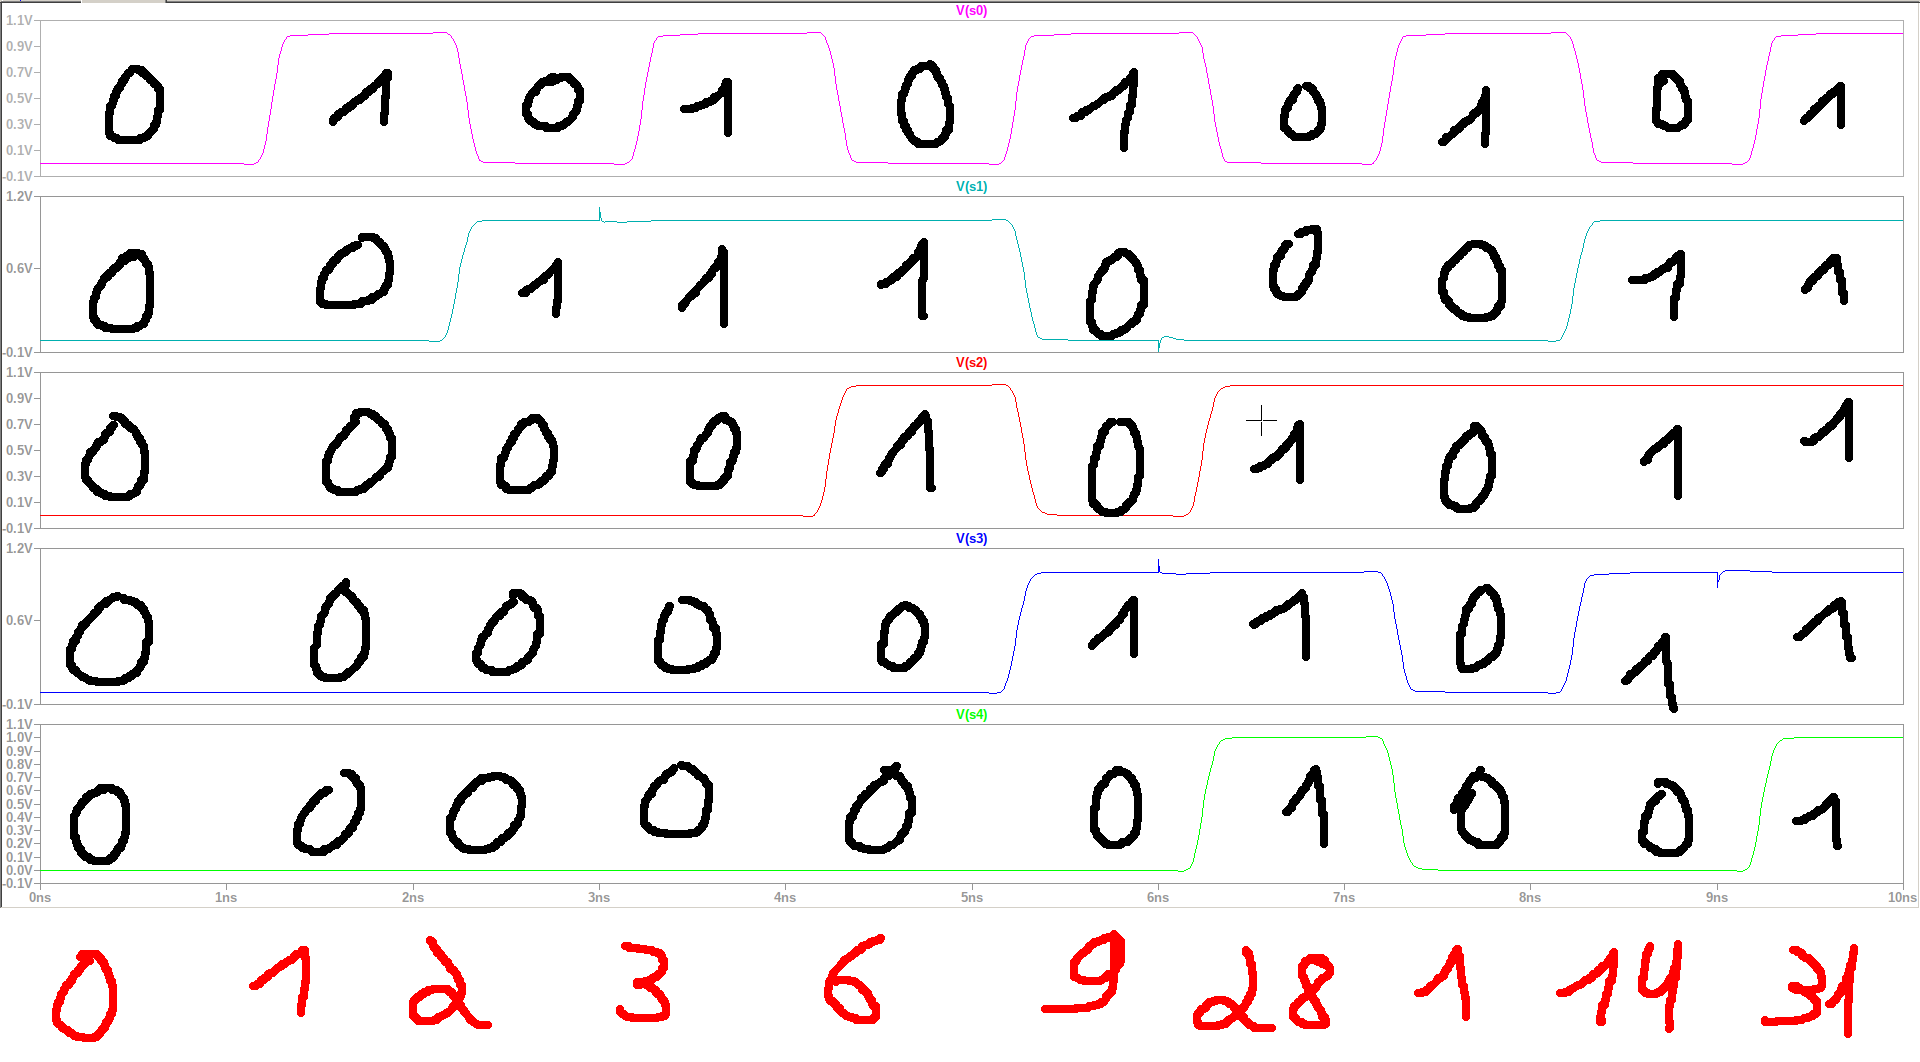
\includegraphics[scale=0.25]{count_bug.png}
    \end{center}
    L'apparition de glitch génère une mauvaise séquence. (Les pulse A0-A4 ont été adapter).
\section{Conclusion}
Les résultats obtenu sont en adéquation avec ceux obtenu lors des simulations LTspice XVII.
On remarque aussi que plus on avance dans la matière de ce cours plus on comprend comment sont implémentés l'architecture de véritables processeurs et leur language assembleur afin de les manipuler et où commence la branche "Programming language theory" de la Science Informatique.

\end{document}
 
